% =====================================================
% Lecture 1 --- Option pricing: motivation and core tools
% =====================================================
\documentclass[10pt,aspectratio=169]{beamer}

% Language & encoding
\usepackage[utf8]{inputenc}
\usepackage[T1]{fontenc}
\usepackage[english]{babel}
\usepackage{lmodern}
\usepackage{microtype}

% Math / tables / layout
\usepackage{amsmath,amssymb,bm,mathtools}
\usepackage{booktabs}
\usepackage{multicol}
\usepackage{changepage}

% Graphics
\usepackage{graphicx}
\usepackage{tikz}
\usetikzlibrary{arrows.meta,positioning,calc,decorations.pathreplacing}
\usepackage{pgfplots}
\pgfplotsset{compat=1.18}

% Theme (Metropolis)
\usetheme[numbering=fraction,progressbar=frametitle]{metropolis}
\setbeamertemplate{frame numbering}[fraction]
\setbeamertemplate{navigation symbols}{}

% Bootcamp palette
\definecolor{BootcampBlueDark}{HTML}{1A3C68}
\definecolor{BootcampBlue}{RGB}{31,110,178}
\definecolor{AccentGold}{HTML}{DAA520}
\definecolor{SoftGray}{RGB}{245,246,248}
\definecolor{TextBlack}{HTML}{000000}
\definecolor{Crimson}{HTML}{990000}
\definecolor{MatrixGreen}{HTML}{228B22}
\definecolor{MatrixRed}{HTML}{B22222}

% Global formatting
\setbeamercolor{normal text}{fg=TextBlack,bg=white}
\setbeamercolor{title}{fg=TextBlack}
\setbeamercolor{structure}{fg=BootcampBlueDark}
\setbeamercolor{progress bar}{fg=BootcampBlueDark,bg=gray!30}

\setbeamercolor{frametitle}{bg=BootcampBlueDark,fg=white}
\setbeamerfont{frametitle}{series=\bfseries,size=\large}
\setbeamertemplate{frametitle}{
  \nointerlineskip
  \begin{beamercolorbox}[wd=\paperwidth,ht=3.2ex,dp=1.4ex,leftskip=1em,rightskip=1em]{frametitle}
    \usebeamerfont{frametitle}\insertframetitle
  \end{beamercolorbox}
}

\setbeamercolor{block title example}{bg=BootcampBlueDark!90!black,fg=white}
\setbeamercolor{block body example}{bg=BootcampBlueDark!5!white,fg=black}
\setbeamercolor{block title proposition}{bg=MatrixGreen!75!black,fg=white}
\setbeamercolor{block body proposition}{bg=MatrixGreen!7!white,fg=black}
\setbeamercolor{block title illustration}{bg=AccentGold!85!black,fg=white}
\setbeamercolor{block body illustration}{bg=AccentGold!10!white,fg=black}
\setbeamercolor{block title proof}{bg=gray!70!black,fg=white}
\setbeamercolor{block body proof}{bg=SoftGray,fg=black}
\setbeamertemplate{blocks}[rounded][shadow=false]

\newenvironment{definitionblock}[1]{%
  \par\vspace{0.4em}%
  \begin{beamercolorbox}[
      wd=\textwidth,sep=0.4em,leftskip=0.3em,rightskip=0.6em,
      rounded=false,shadow=false
    ]{block title example}%
    \raisebox{0.15em}{\usebeamerfont{block title example}#1}%
  \end{beamercolorbox}%
  \vspace{-0.4em}%
  \begin{beamercolorbox}[
      wd=\textwidth,sep=0.9em,leftskip=0.6em,rightskip=0.6em,
      rounded=false,shadow=false
    ]{block body example}%
    \usebeamerfont{block body example}%
}{%
  \end{beamercolorbox}%
  \par\vspace{0.6em}%
}

\newenvironment{propositionblock}[1]{%
  \par\vspace{0.35em}%
  \begin{beamercolorbox}[
      wd=\textwidth,sep=0.4em,leftskip=0.3em,rightskip=0.6em,
      rounded=false,shadow=false
    ]{block title proposition}%
    \raisebox{0.15em}{\usebeamerfont{block title example}#1}%
  \end{beamercolorbox}%
  \vspace{-0.4em}%
  \begin{beamercolorbox}[
      wd=\textwidth,sep=0.8em,leftskip=0.6em,rightskip=0.6em,
      rounded=false,shadow=false
    ]{block body proposition}%
    \usebeamerfont{block body example}%
}{%
  \end{beamercolorbox}%
  \par\vspace{0.55em}%
}

\newenvironment{illustrationblock}[1]{%
  \par\vspace{0.35em}%
  \begin{beamercolorbox}[
      wd=\textwidth,sep=0.4em,leftskip=0.3em,rightskip=0.6em,
      rounded=false,shadow=false
    ]{block title illustration}%
    \raisebox{0.15em}{\usebeamerfont{block title example}#1}%
  \end{beamercolorbox}%
  \vspace{-0.4em}%
  \begin{beamercolorbox}[
      wd=\textwidth,sep=0.8em,leftskip=0.6em,rightskip=0.6em,
      rounded=false,shadow=false
    ]{block body illustration}%
    \usebeamerfont{block body example}%
}{%
  \end{beamercolorbox}%
  \par\vspace{0.55em}%
}

\newenvironment{proofblock}[1]{%
  \par\vspace{0.3em}%
  \begin{beamercolorbox}[
      wd=\textwidth,sep=0.35em,leftskip=0.3em,rightskip=0.6em,
      rounded=false,shadow=false
    ]{block title proof}%
    \raisebox{0.15em}{\usebeamerfont{block title example}#1}%
  \end{beamercolorbox}%
  \vspace{-0.4em}%
  \begin{beamercolorbox}[
      wd=\textwidth,sep=0.7em,leftskip=0.6em,rightskip=0.6em,
      rounded=false,shadow=false
    ]{block body proof}%
    \usebeamerfont{block body example}%
}{%
  \end{beamercolorbox}%
  \par\vspace{0.45em}%
}

% One compact transition slide per major section. Subsections remain visible
% in the source structure without adding extra transition pages.
\AtBeginSection[]{
  \begin{frame}{\insertsectionhead}
    \small
    \tableofcontents[currentsection,sectionstyle=show/hide,hideothersubsections]
  \end{frame}
}

\graphicspath{{bm_figs/}}

% Metadata
\title{Option Pricing: Motivation and First Mathematical Tools}
\author{}
\date{}

\begin{document}

\begin{frame}[plain]
  \vfill
  {\usebeamerfont{title}\usebeamercolor[fg]{title}\inserttitle\par}
  \medskip
  {\color{BootcampBlueDark}\rule{0.95\textwidth}{0.8pt}}
  \vfill
\end{frame}

\begin{frame}{How the course materials fit together}
\small
\begin{columns}[T,onlytextwidth]
  \begin{column}{0.31\textwidth}
    \begin{definitionblock}{Slides}
      \raggedright The in-class : core ideas, examples, and formulas.
    \end{definitionblock}
  \end{column}
  \begin{column}{0.31\textwidth}
    \begin{propositionblock}{Lecture notes}
      \raggedright The full reference: definitions, derivations, proofs, and worked examples.
    \end{propositionblock}
  \end{column}
  \begin{column}{0.31\textwidth}
    \begin{illustrationblock}{Exercises and HW}
      \raggedright The practice layer: calculations, code...
    \end{illustrationblock}
  \end{column}
\end{columns}

\end{frame}
\begin{frame}{Homework and final grade}
\scriptsize

\begin{columns}[T,onlytextwidth]
  \begin{column}{0.48\textwidth}
    \begin{block}{Homework rhythm}
      \begin{itemize}\setlength{\itemsep}{0.12em}
        \item Homework is assigned \textbf{weekly}; you have \textbf{two weeks}
        to complete each assignment. Brightspace gives the official deadline
        and submission instructions.
        \item \textbf{Practice assignments:} mathematical reasoning and calculations.
        \item \textbf{Numerical assignments:} simulation or approximation,
        with code and interpretation.
        \item The \textbf{lowest homework score is dropped}.
      \end{itemize}
    \end{block}
  \end{column}

  \begin{column}{0.48\textwidth}
    \begin{block}{Two grading routes}
      \centering
      \renewcommand{\arraystretch}{0.95}
      \begin{tabular}{@{}lcc@{}}
        \toprule
        & \textbf{Grade 1} & \textbf{Grade 2} \\
        \midrule
        Homework average & 50\% & 60\% \\
        Midterm exam     & 20\% & 0\%  \\
        Final exam       & 30\% & 40\% \\
        \bottomrule
      \end{tabular}

      \vspace{0.35em}
      {\normalsize
      $\text{Final Grade}=\max\bigl(\text{Grade 1},\text{Grade 2}\bigr)$
      }\par
      \vspace{0.1em}
      The more favorable calculation is used automatically.
    \end{block}
  \end{column}
\end{columns}

\vspace{-0.15em}

\begin{block}{Letter-grade scale}
\centering
\scriptsize
\renewcommand{\arraystretch}{0.95}
\begin{tabular}{@{}ccccccccccc@{}}
\toprule
\textbf{F} & \textbf{D} & \textbf{D+} & \textbf{C-} &
\textbf{C} & \textbf{C+} & \textbf{B-} & \textbf{B} &
\textbf{B+} & \textbf{A-} & \textbf{A} \\
\midrule
$<62.45$ &
$62.45$ &
$66.45$ &
$69.45$ &
$72.45$ &
$76.45$ &
$79.45$ &
$82.45$ &
$86.45$ &
$89.45$ &
$94.45$ \\
\bottomrule
\end{tabular}

\vspace{0.05em}
\textit{Each value indicates the minimum percentage required for that letter grade.}
\end{block}

\end{frame}

\begin{frame}{References (see Brightspaces)}
\footnotesize
\textbf{Main references}
\begin{itemize}\setlength{\itemsep}{0.5em}
  \item S.~Shreve, \emph{Stochastic Calculus for Finance II}, Chapters 1--2.
  \item I.~Karatzas and S.~Shreve, \emph{Brownian Motion and Stochastic Calculus}, Chapter 1.
  \item S.~Shreve, \emph{Stochastic Calculus for Finance I}, Chapters 1--2 for discrete-time pricing intuition.
\end{itemize}
\end{frame}

\begin{frame}{Roadmap}
  \tableofcontents[hideallsubsections]
\end{frame}

% =====================================================
\section{Motivation, replication, and pricing}
\subsection{Contracts and time value}

\begin{frame}{Derivatives reshape future financial risk}
\begin{itemize}
  \item An airline is exposed to future fuel prices; an exporter is exposed to exchange rates.\pause
  \item A \textbf{financial contract} specifies future cash flows between two parties.\pause
  \item A \textbf{derivative} links those cash flows to an observable market quantity.\pause
\end{itemize}

\begin{block}{The pricing question}
What amount paid \textbf{today} is consistent with a possibly random \textbf{future payoff}?
\end{block}
\end{frame}

\begin{frame}{One option introduces most of the vocabulary}
Suppose a one-year call option on a stock has strike $K=100$:
\[
X=(S_T-K)^+=(S_T-100)^+.
\]

\begin{itemize}
  \item $S$ is the \textbf{underlying}; $T$ is the \textbf{maturity}.\pause
  \item $X$ is the \textbf{payoff}: its rule is known today and its value is realized at $T$.\pause
  \item The \textbf{long} pays the option price today and receives $X$ at $T$.\pause
  \item The \textbf{short} receives the price today and owes $X$ at $T$.
\end{itemize}

If $S_T=125$, then $X=25$; if $S_T=90$, then $X=0$.
\end{frame}

\begin{frame}{A dollar today and a dollar tomorrow are different}
At a constant continuously compounded rate $r$, the bank account is $B_t=e^{rt}$.

\begin{definitionblock}{Discounting}
A certain payment of $C$ at time $T$ has value
\[
C e^{-rT}
\]
today, because this amount invested in the bank account produces exactly $C$ at $T$.
\end{definitionblock}

\begin{illustrationblock}{Example}
If $C=100$, $r=5\%$, and $T=1$, the present value is
\[
100e^{-0.05}\approx95.12.
\]
\end{illustrationblock}
\end{frame}

\subsection{The casino reveals the role of replication}

\begin{frame}{Historical expectation is a natural first guess}
I sell a contract with payoff
\[
X=
\begin{cases}
\$100,&\text{if red occurs},\\
\$0,&\text{if black occurs}.
\end{cases}
\]
Under the historical probability measure $\mathbb P$,
\[
\mathbb P(\text{red})=0.99,
\qquad
\mathbb P(\text{black})=0.01,
\]
so
\[
\mathbb E^{\mathbb P}[X]
=0.99\times\$100+0.01\times\$0
=\$99.
\]

\begin{block}{Pricing question}
Is $\$99$ the arbitrage-free price? \textbf{No.} Historical probabilities describe likelihoods; they do not by themselves price a replicable claim.
\end{block}
\end{frame}

\begin{frame}{A $\$50$ bet reproduces the contract state by state}
\begin{center}
\large What payoff does $\$50$ placed on red produce?
\end{center}

\begin{center}
\renewcommand{\arraystretch}{1.4}
\begin{tabular}{@{}lcc@{}}
\toprule
 & Red & Black \\
\midrule
Contract & $\$100$ & $\$0$ \\
$\$50$ bet on red & $2\times\$50=\$100$ & $\$0$ \\
\bottomrule
\end{tabular}
\end{center}

\[
\text{same terminal payoff in every state}
\quad\Longrightarrow\quad
\text{replication cost}=\$50.
\]

\begin{propositionblock}{Takeaway}
\centering
\textbf{PRICE = COST OF REPLICATION}
\end{propositionblock}
\end{frame}

\begin{frame}{No arbitrage forces the price to be $\$50$}
\[
C_0=\$50,
\qquad\text{not}\qquad
\mathbb E^{\mathbb P}[X]=\$99.
\]

\begin{columns}[T,onlytextwidth]
\column{0.47\textwidth}
\textbf{If the contract costs more than $\$50$}
\begin{itemize}
  \item sell the contract;
  \item buy the $\$50$ hedge;
  \item keep the difference with no terminal risk.
\end{itemize}

\column{0.47\textwidth}
\textbf{If it costs less than $\$50$}
\begin{itemize}
  \item buy the contract;
  \item sell the replicating bet;
  \item keep the reverse difference.
\end{itemize}
\end{columns}

\begin{block}{Transition}
Historical probabilities describe likelihoods. Which probabilities represent prices consistently with traded assets?
\end{block}
\end{frame}

\subsection{A one-period financial market}

\begin{frame}{A one-period stock model makes replication visible}
Assume a zero interest rate. A stock is worth $S_0=50$ today and
\[
S_1=
\begin{cases}
60 & \text{up},\\
40 & \text{down}.
\end{cases}
\]
A call with strike $K=50$ pays
\[
X=(S_1-50)^+
=\begin{cases}10&\text{up},\\0&\text{down}.\end{cases}
\]

\begin{center}
Can stock and cash reproduce both payoffs?
\end{center}
\end{frame}

\begin{frame}{Worked example: replication determines the call price}
Hold $\Delta$ shares and $b$ dollars in cash. Matching both terminal payoffs gives
\[
60\Delta+b=10,
\qquad
40\Delta+b=0.
\]
Therefore
\[
\Delta=\tfrac12,
\qquad b=-20,
\qquad
V_0=\Delta S_0+b=5.
\]

\begin{propositionblock}{Law of one price}
The call and its replicating portfolio have the same payoff in every state, so both must cost $5$ today.
\end{propositionblock}
\end{frame}

\begin{frame}{Risk-neutral probabilities encode the same restriction}
Choose $q=\mathbb Q(\text{up})$ so that the stock has no drift at zero interest:
\[
50=q\times60+(1-q)\times40
\quad\Longrightarrow\quad q=\tfrac12.
\]
Then
\[
V_0=\mathbb E^{\mathbb Q}[X]
=\tfrac12\times10+\tfrac12\times0=5.
\]

\begin{block}{Interpretation}
The physical probability may differ from $q$. Replication determines the price first; the risk-neutral expectation is its mathematical representation.
\end{block}
\end{frame}

\begin{frame}{Student exercise: replicate a similar call}
Assume a zero interest rate. A stock is worth $S_0=100$ and
\[
S_1=125\ \text{or}\ 75.
\]
A call with strike $K=100$ pays $25$ or $0$.

\begin{enumerate}
  \item Write the two replication equations for $(\Delta,b)$.
  \item Find the no-arbitrage call price.
  \item Find the risk-neutral up probability.
  \item Explain why the physical up probability is unnecessary.
\end{enumerate}

\begin{block}{Hint}
Subtract the two payoff equations before solving for cash.
\end{block}
\end{frame}

\begin{frame}{Solution: replication and risk-neutral probability}
Matching the two terminal payoffs gives
\[
125\Delta+b=25,
\qquad
75\Delta+b=0.
\]
Subtracting the equations,
\[
\Delta=\frac{25}{125-75}=\frac12,
\qquad
b=-37.5.
\]
Hence the replication cost is
\[
V_0=\Delta S_0+b
=\frac12\times100-37.5
=12.5.
\]
The risk-neutral probability solves
\[
100=125q+75(1-q),
\qquad q=\frac12,
\]
and therefore $\mathbb E^{\mathbb Q}[X]=12.5$. The physical up probability is not needed.
\end{frame}

\begin{frame}{Replication motivates the tools used throughout the course}
For a replicable payoff $X$, an arbitrage-free model represents its value as
\[
V_t=B_t\,\mathbb E^{\mathbb Q}\!\left[
\frac{X}{B_T}\,\middle|\,\mathcal F_t
\right].
\]

To understand this expression, we now build a probability toolbox in layers:
\[
\text{distribution}
\longrightarrow
\text{expectation}
\longrightarrow
\text{information}
\longrightarrow
\text{conditional prediction}
\longrightarrow
\text{martingale}.
\]
\end{frame}

% =====================================================
\section{Probability toolbox}
\subsection{Random variables, distributions, CDFs, and densities}

\begin{frame}{Introductory example: a payoff is a random variable}
Suppose the terminal stock price has the following physical distribution:
\[
\begin{array}{c|ccc}
S_T & 80 & 100 & 130 \\ \hline
\mathbb P & 0.20 & 0.50 & 0.30
\end{array}
\]
For a call with strike $K=100$, $X=(S_T-100)^+$:
\[
\begin{array}{c|ccc}
S_T & 80 & 100 & 130 \\ \hline
X   & 0  & 0   & 30
\end{array}
\]

The payoff rule maps each state to a number; the probabilities of those numbers form the \textbf{distribution of $X$}.
\end{frame}

\begin{frame}{Definitions: random variable and distribution}
\begin{definitionblock}{Random variable and its law}
A random variable is a measurable map
\[
X:(\Omega,\mathcal F)\longrightarrow(\mathbb R,\mathcal B(\mathbb R)).
\]
It assigns a numerical outcome to every state. Its distribution, or law, is
\[
\mathbb P_X(A)=\mathbb P(X\in A),
\qquad A\in\mathcal B(\mathbb R).
\]
\end{definitionblock}

The random variable is the state-to-number rule; its distribution records how likely its possible values are.
\end{frame}

\begin{frame}{The CDF accumulates probability from left to right}
\begin{definitionblock}{Cumulative distribution function}
\[
F_X(x)=\mathbb P(X\le x).
\]
\end{definitionblock}

Every CDF is nondecreasing, right-continuous, and satisfies
\[
\lim_{x\to-\infty}F_X(x)=0,
\qquad
\lim_{x\to\infty}F_X(x)=1.
\]

Probabilities of intervals follow from differences:
\[
\mathbb P(a<X\le b)=F_X(b)-F_X(a).
\]

\begin{block}{Do not confuse the objects}
The \textbf{distribution} is a probability measure; the \textbf{CDF} is its cumulative function; a \textbf{density} is a derivative when one exists.
\end{block}
\end{frame}

\begin{frame}{Worked example: the exponential CDF comes from its density}
Let $X\sim\operatorname{Exp}(\lambda)$ with
\[
f_X(x)=\lambda e^{-\lambda x}\mathbf 1_{\{x\ge0\}}.
\]
Then, for $x\ge0$,
\[
F_X(x)=\int_{-\infty}^{x}f_X(u)\,du
=\int_0^x\lambda e^{-\lambda u}\,du
=1-e^{-\lambda x}.
\]
Thus
\[
\mathbb P(a<X\le b)=e^{-\lambda a}-e^{-\lambda b},
\qquad 0\le a<b.
\]

When differentiability holds,
\[
f_X(x)=F_X'(x).
\]
\end{frame}

%\begin{frame}{Student exercise: build the CDF of a one-day return}
%A stock's one-day return $R$ satisfies
%\[
%\mathbb P(R=-2\%)=0.40,
%\qquad
%\mathbb P(R=3\%)=0.60.
%\]
%
%\begin{enumerate}
%  \item List the possible values and probabilities of $R$.
%  \item Compute $F_R(r)=\mathbb P(R\le r)$ on the whole real line.
%  \item Use the CDF to find $\mathbb P(R>0)$.
%  \item Where does the CDF jump, and by how much?
%\end{enumerate}
%
%\begin{block}{Hint}
%A discrete CDF is a step function; each jump equals the probability at that value.
%\end{block}
%\end{frame}
%
%\begin{frame}{Solution: the return CDF is a step function}
%The CDF is
%\[
%F_R(r)=
%\begin{cases}
%0, & r<-2\%,\\
%0.40, & -2\%\le r<3\%,\\
%1, & r\ge3\%.
%\end{cases}
%\]
%Since $0$ lies between the two possible returns,
%\[
%\mathbb P(R>0)
%=1-F_R(0)
%=1-0.40
%=0.60.
%\]
%
%\begin{propositionblock}{Reading the graph}
%The jump at $-2\%$ has size $0.40$; the jump at $3\%$ has size $0.60$.
%\end{propositionblock}
%\end{frame}

\subsection{Expectation, variance, and dependence}

\begin{frame}{Definition: expectation is a probability-weighted average}
\begin{definitionblock}{Expectation}
For an integrable random variable $X$,
\[
\mathbb E[X]=\sum_x x\,\mathbb P(X=x)
\quad\text{or}\quad
\mathbb E[X]=\int_{\mathbb R}x f_X(x)\,dx.
\]
Integrable means $\mathbb E[|X|]<\infty$, written $X\in L^1$.
\end{definitionblock}

Expectation uses a distribution to summarize the long-run or model-based average. It has the same financial unit as $X$.
\end{frame}

\begin{frame}{Functions of a random variable can be averaged directly}
\begin{propositionblock}{Averaging a transformation}
For measurable $g$, whenever the expectation exists,
\[
\mathbb E[g(X)]
=\sum_x g(x)\mathbb P(X=x)
\quad\text{or}\quad
\mathbb E[g(X)]=\int_{\mathbb R}g(x)f_X(x)\,dx.
\]
\end{propositionblock}

\begin{illustrationblock}{Indicator payoff}
For $X=\mathbf 1_A$,
\[
\mathbb E[X]=\mathbb P(A).
\]
This is why a digital payoff is naturally connected to an event probability.
\end{illustrationblock}
\end{frame}

\begin{frame}{Proposition: expectation is linear and respects order}
For $X,Y\in L^1$ and $a,b\in\mathbb R$,
\begin{propositionblock}{Fundamental properties}
\begin{align*}
\mathbb E[aX+bY]&=a\mathbb E[X]+b\mathbb E[Y],\\
X\ge0&\Longrightarrow\mathbb E[X]\ge0,\\
X\le Y&\Longrightarrow\mathbb E[X]\le\mathbb E[Y],\\
|\mathbb E[X]|&\le\mathbb E[|X|].
\end{align*}
\end{propositionblock}

Linearity does not require independence. Independence matters when variances and products are calculated.
\end{frame}

\begin{frame}{Variance measures dispersion around the mean}
\begin{definitionblock}{Mean, second moment, and variance}
\[
\mu=\mathbb E[X],
\qquad
m_2=\mathbb E[X^2],
\qquad
\operatorname{Var}(X)=\mathbb E[(X-\mu)^2].
\]
The standard deviation is $\operatorname{SD}(X)=\sqrt{\operatorname{Var}(X)}$.
\end{definitionblock}

\begin{propositionblock}{Useful identity}
\[
\operatorname{Var}(X)=\mathbb E[X^2]-\mathbb E[X]^2.
\]
\end{propositionblock}

Mean describes location; variance describes uncertainty around that location.
\end{frame}

\begin{frame}{Covariance links dependence to portfolio variance}
\begin{definitionblock}{Covariance}
\[
\operatorname{Cov}(X,Y)
=\mathbb E[(X-\mathbb E[X])(Y-\mathbb E[Y])].
\]
\end{definitionblock}

\begin{propositionblock}{Variance of a linear combination}
\[
\operatorname{Var}(aX+bY)
=a^2\operatorname{Var}(X)+b^2\operatorname{Var}(Y)
+2ab\operatorname{Cov}(X,Y).
\]
If $X$ and $Y$ are independent, then $\operatorname{Cov}(X,Y)=0$.
\end{propositionblock}

This identity explains why dependence matters when risks are combined.
\end{frame}

\begin{frame}{Reference: classical means and variances to know}
\small
\renewcommand{\arraystretch}{1.28}
\begin{center}
\begin{tabular}{@{}lccc@{}}
\toprule
Law of $X$ & Parameters & $\mathbb E[X]$ & $\operatorname{Var}(X)$ \\
\midrule
Bernoulli & $p$ & $p$ & $p(1-p)$ \\
Binomial & $n,p$ & $np$ & $np(1-p)$ \\
Poisson & $\lambda$ & $\lambda$ & $\lambda$ \\
Uniform & $[a,b]$ & $(a+b)/2$ & $(b-a)^2/12$ \\
Exponential & rate $\lambda$ & $1/\lambda$ & $1/\lambda^2$ \\
Gaussian & $\mu,\sigma^2$ & $\mu$ & $\sigma^2$ \\
\bottomrule
\end{tabular}
\end{center}

The exercise sheet contains the detailed derivations; class time focuses on choosing the right representation.
\end{frame}

\begin{frame}{Example A: derive discrete moments together}
Let $B_1,\ldots,B_n$ be independent Bernoulli$(p)$ variables and set
\[
N_n=\sum_{k=1}^n B_k.
\]

\begin{enumerate}
  \item Use $B_k^2=B_k$ to find $\mathbb E[B_k]$ and $\operatorname{Var}(B_k)$.
  \item Use linearity to find $\mathbb E[N_n]$.
  \item Where is independence used to find $\operatorname{Var}(N_n)$?
\end{enumerate}

\begin{block}{Progressive hint}
Write the variance of the sum using covariance terms before setting them to zero.
\end{block}
\end{frame}

\begin{frame}{Solution: moments of a Bernoulli sum}
For $B_k\sim\operatorname{Bernoulli}(p)$,
\[
B_k^2=B_k,
\qquad
\mathbb E[B_k]=p,
\qquad
\operatorname{Var}(B_k)=p-p^2=p(1-p).
\]
Linearity gives
\[
\mathbb E[N_n]
=\sum_{k=1}^n\mathbb E[B_k]
=np.
\]
Independence makes all cross-covariances vanish, so
\[
\operatorname{Var}(N_n)
=\sum_{k=1}^n\operatorname{Var}(B_k)
=np(1-p).
\]

\begin{block}{Where independence enters}
It is not needed for the mean; it is used when simplifying the variance of the sum.
\end{block}
\end{frame}

\begin{frame}{Exercise B: derive continuous moments independently}
Choose one variable and justify every step.

\begin{enumerate}
  \item If $U\sim\operatorname{Unif}[a,b]$, compute $\mathbb E[U]$, $\mathbb E[U^2]$, and $\operatorname{Var}(U)$.
  \item If $T\sim\operatorname{Exp}(\lambda)$, compute the same three quantities using integration by parts.
  \item For $Z\sim\mathcal N(0,1)$, use symmetry to identify which odd moments vanish.
\end{enumerate}

\begin{block}{Extension}
For $X\sim\operatorname{Poisson}(\lambda)$, start from $\mathbb E[X(X-1)]$ rather than expanding $X^2$ directly.
\end{block}
\end{frame}

\begin{frame}{Solution: classical moment calculations}
\small
\renewcommand{\arraystretch}{1.45}
\begin{center}
\begin{tabular}{@{}lccc@{}}
\toprule
Law & $\mathbb E[X]$ & $\mathbb E[X^2]$ & $\operatorname{Var}(X)$ \\
\midrule
$U\sim\operatorname{Unif}[a,b]$
& $\dfrac{a+b}{2}$
& $\dfrac{a^2+ab+b^2}{3}$
& $\dfrac{(b-a)^2}{12}$ \\
$T\sim\operatorname{Exp}(\lambda)$
& $\dfrac1\lambda$
& $\dfrac{2}{\lambda^2}$
& $\dfrac1{\lambda^2}$ \\
\bottomrule
\end{tabular}
\end{center}

For $Z\sim\mathcal N(0,1)$, symmetry gives
\[
\mathbb E[Z^{2m+1}]=0
\qquad (m\ge0).
\]
For $X\sim\operatorname{Poisson}(\lambda)$,
\[
\mathbb E[X(X-1)]=\lambda^2
\quad\Longrightarrow\quad
\mathbb E[X^2]=\lambda^2+\lambda,
\quad
\operatorname{Var}(X)=\lambda.
\]
\end{frame}

\subsection{Sample averages, LLN, and CLT}

\begin{frame}{A sample summarizes repeated observations}
Let $X_1,\ldots,X_n$ be observations of the same quantity. Define
\begin{definitionblock}{Empirical mean and empirical variance}
\[
\overline X_n=\frac1n\sum_{i=1}^n X_i,
\qquad
v_n=\frac1n\sum_{i=1}^n (X_i-\overline X_n)^2.
\]
\end{definitionblock}

$\overline X_n$ estimates the population mean and $v_n$ its variance. The unbiased sample variance is
\[
s_n^2=\frac{n}{n-1}v_n.
\]

These statistics will later summarize samples of returns, losses, and simulated payoffs.
\end{frame}

\begin{frame}{The LLN finds the target; the CLT describes the error}
\small
Let $X_1,X_2,\ldots$ be i.i.d. with mean $\mu$.
\begin{propositionblock}{Law of Large Numbers}
If $\mathbb E[|X_1|]<\infty$, then
\[
\overline X_n\longrightarrow \mu=\mathbb E[X_1]
\quad\text{in probability.}
\]
\end{propositionblock}

If also $0<\sigma^2=\operatorname{Var}(X_1)<\infty$,
\begin{propositionblock}{Central Limit Theorem}
\[
\frac{\sqrt n\,(\overline X_n-\mu)}{\sigma}
\xRightarrow[n\to\infty]{}\mathcal N(0,1)
\quad\text{in law.}
\]
\end{propositionblock}

The LLN says the error vanishes; the CLT says its typical size is $\sigma/\sqrt n$ and gives its approximate shape.
\end{frame}

\begin{frame}{Worked example: estimate a success probability}
Let $X_i\sim\operatorname{Bernoulli}(0.60)$ independently and let $\overline X_{100}$ be the success frequency in $100$ trials.
\[
\mathbb E[\overline X_{100}]=0.60,
\qquad
\operatorname{SD}(\overline X_{100})
=\sqrt{\frac{0.60(0.40)}{100}}
\approx0.049.
\]
The LLN explains why the frequency should be near $0.60$. The CLT gives
\[
\mathbb P(0.50\le \overline X_{100}\le0.70)
\approx
\mathbb P(-2.04\le Z\le2.04)
\approx0.96.
\]

\begin{illustrationblock}{Why it matters}
Averages stabilize, but their residual sampling uncertainty is of order $1/\sqrt n$.
\end{illustrationblock}
\end{frame}

%\begin{frame}{Student exercise: use the CLT for an average loss}
%Daily losses $X_1,\ldots,X_{225}$ are i.i.d. with
%\[
%\mathbb E[X_i]=2,
%\qquad
%\operatorname{SD}(X_i)=3.
%\]
%
%\begin{enumerate}
%  \item What value does $\overline X_{225}$ approach according to the LLN?
%  \item What is the standard deviation of $\overline X_{225}$?
%  \item Use the CLT to approximate $\mathbb P(\overline X_{225}>2.4)$.
%\end{enumerate}
%
%\begin{block}{Hint}
%Standardize $2.4$ using the standard error $\sigma/\sqrt n$.
%\end{block}
%\end{frame}

%\begin{frame}{Solution: the average fluctuates on a $1/\sqrt n$ scale}
%The LLN gives $\overline X_{225}\to2$ in probability. Moreover,
%\[
%\operatorname{SD}(\overline X_{225})
%=\frac{3}{\sqrt{225}}=0.2.
%\]
%Therefore the CLT yields
%\[
%\mathbb P(\overline X_{225}>2.4)
%\approx
%\mathbb P\!\left(Z>\frac{2.4-2}{0.2}\right)
%=\mathbb P(Z>2)
%\approx0.023.
%\]
%
%\begin{propositionblock}{Interpretation}
%The LLN identifies the limiting center $2$; the CLT quantifies a finite-sample deviation from that center.
%\end{propositionblock}
%\end{frame}

\subsection{Characteristic functions and joint distributions}

\begin{frame}{Characteristic functions encode an entire distribution}
\begin{definitionblock}{Characteristic function}
\[
\varphi_X(u)=\mathbb E[e^{iuX}],
\qquad u\in\mathbb R.
\]
\end{definitionblock}

\begin{itemize}
  \item $|e^{iuX}|=1$, so $\varphi_X$ always exists.
  \item The characteristic function uniquely determines the distribution.
  \item It turns probability calculations into Fourier calculations.
  \item Unlike a moment generating function, it does not require exponential moments.
\end{itemize}

This is a recognition tool for later work, not a full Fourier theory.
\end{frame}

\begin{frame}{Independent sums become products in Fourier space}
If $X$ and $Y$ are independent,
\begin{propositionblock}{Product rule}
\[
\varphi_{X+Y}(u)=\varphi_X(u)\varphi_Y(u).
\]
\end{propositionblock}

For $Z\sim\mathcal N(0,1)$,
\[
\varphi_Z(u)=e^{-u^2/2}.
\]
Thus, for independent standard normals $Z_1,Z_2$,
\[
\varphi_{Z_1+Z_2}(u)=e^{-u^2},
\]
which identifies $Z_1+Z_2\sim\mathcal N(0,2)$.
\end{frame}

\begin{frame}{Joint distributions describe dependence between variables}
Consider
\[
\begin{array}{c|cc|c}
 & Y=0 & Y=1 & \mathbb P_X \\ \hline
X=0 & 0.30 & 0.10 & 0.40 \\
X=1 & 0.20 & 0.40 & 0.60 \\ \hline
\mathbb P_Y & 0.50 & 0.50 & 1
\end{array}
\]

\begin{itemize}
  \item The four interior values form the \textbf{joint distribution}.
  \item Row and column sums are the \textbf{marginal distributions}.
  \item The joint law tells us how observing one variable changes what we know about the other.
\end{itemize}

This observation creates the need for information and conditional distributions.
\end{frame}

% =====================================================
\section{Information and conditional expectation}
\subsection{Information first, formalism second}

\begin{frame}{Introductory example: observing a signal reveals a partition}
A fair die produces the full outcome $X(\omega)=\omega$. Instead of observing $X$, we observe only
\[
Y=\mathbf 1_{\{X\text{ is even}\}}.
\]

Knowing $Y$ tells us which information set contains the outcome:
\[
O=\{1,3,5\},
\qquad
E=\{2,4,6\}.
\]

\begin{itemize}
  \item $Y$ distinguishes odd from even outcomes.
  \item $Y$ cannot distinguish $2$ from $4$ or $6$.
  \item Observing $Y$ therefore reveals the partition $\{O,E\}$.
\end{itemize}
\end{frame}

\begin{frame}{The notation $\sigma(Y)$ records exactly what $Y$ reveals}
After observing the parity signal $Y$, we can decide whether
\[
\omega\in O,\qquad
\omega\in E,\qquad
\omega\in\Omega,\qquad
\omega\in\emptyset.
\]
We cannot decide whether $\omega=2$, because $Y$ gives the same signal for $2$, $4$, and $6$.

\begin{definitionblock}{Information generated by a random variable}
\[
\sigma(Y)
=\{\text{events whose occurrence can be determined from }Y\}.
\]
For this example,
\[
\sigma(Y)=\{\emptyset,O,E,\Omega\}.
\]
\end{definitionblock}

Thus $\sigma(Y)$ is the information revealed by observing $Y$, written as a collection of observable events.
\end{frame}

\begin{frame}{A sigma-algebra formalizes observable yes-or-no questions}
\begin{definitionblock}{$\sigma$-algebra}
A collection $\mathcal G$ of events is a $\sigma$-algebra if
\begin{itemize}
  \item $\Omega\in\mathcal G$;
  \item $A\in\mathcal G$ implies $A^c\in\mathcal G$;
  \item $A_1,A_2,\ldots\in\mathcal G$ implies $\bigcup_n A_n\in\mathcal G$.
\end{itemize}
\end{definitionblock}

The closure rules ensure that observable questions can be combined consistently.
\end{frame}

\begin{frame}{Measurable means determined by the available information}
\begin{definitionblock}{$\mathcal G$-measurable random variable}
A random variable $Z$ is $\mathcal G$-measurable if
\[
\{Z\in B\}\in\mathcal G
\qquad\text{for every Borel set }B.
\]
\end{definitionblock}

\begin{block}{Information interpretation}
``$Z$ is $\mathcal G$-measurable'' means that the information in $\mathcal G$ is sufficient to determine $Z$.
\end{block}

In a finite model,
\[
Z\text{ is }\sigma(Y)\text{-measurable}
\quad\Longleftrightarrow\quad
Z=g(Y)\text{ for some function }g.
\]
Thus $Z$ must take the same value whenever $Y$ takes the same value.
\end{frame}

\begin{frame}{Worked example: measurable quantities are constant on signal sets}
For the parity signal, a $\sigma(Y)$-measurable variable has the form
\[
Z=a\mathbf 1_O+b\mathbf 1_E.
\]

\begin{itemize}
  \item $Z_1=10\cdot\mathbf 1_E$ is measurable: parity determines it.
  \item $Z_2=X$ is not measurable: parity does not determine the die value.
  \item $Z_3=(-1)^X$ is measurable: it is a function of parity.
\end{itemize}

\begin{propositionblock}{Finite-state test}
A variable is measurable with respect to the observed partition if and only if it is constant on every information set.
\end{propositionblock}
\end{frame}

\begin{frame}{Student exercise: what does a coarse price signal reveal?}
A terminal stock price takes values $80$, $100$, or $130$. The signal is
\[
Y=\mathbf 1_{\{S_T\ge100\}}.
\]

\begin{enumerate}
  \item Write the partition generated by observing $Y$.
  \item List the events in $\sigma(Y)$.
  \item Is the call payoff $(S_T-100)^+$ measurable with respect to $\sigma(Y)$?
  \item Is the digital payoff $\mathbf 1_{\{S_T\ge100\}}$ measurable?
\end{enumerate}

\begin{block}{Test}
Can two states with the same signal produce different values of the quantity?
\end{block}
\end{frame}

\begin{frame}{Solution: the signal groups states with the same observation}
The signal distinguishes the two information sets
\[
\{80\}
\qquad\text{and}\qquad
\{100,130\}.
\]
Hence
\[
\sigma(Y)
=\{\emptyset,\Omega,\{80\},\{100,130\}\}.
\]
The call payoff takes values $0$ and $30$ inside $\{100,130\}$, so it is \textbf{not} $\sigma(Y)$-measurable.

The digital payoff equals the signal:
\[
\mathbf 1_{\{S_T\ge100\}}=Y,
\]
so it is $\sigma(Y)$-measurable.

\begin{block}{Test}
The signal determines a quantity exactly if that quantity is constant on every information set.
\end{block}
\end{frame}

\subsection{Conditional distributions and conditional expectation}

\begin{frame}{A conditional distribution updates the relevant probabilities}
Return to the joint distribution
\[
\begin{array}{c|cc}
 & Y=0 & Y=1 \\ \hline
X=0 & 0.30 & 0.10 \\
X=1 & 0.20 & 0.40
\end{array}
\]
Since $\mathbb P(Y=1)=0.50$,
\[
\mathbb P(X=1\mid Y=1)
=\frac{\mathbb P(X=1,Y=1)}{\mathbb P(Y=1)}
=\frac{0.40}{0.50}=0.80.
\]

Observing $Y=1$ replaces the marginal law of $X$ by the conditional law of $X$ given that information.
\end{frame}

\begin{frame}{Conditional expectation is the best prediction from current information}
\begin{block}{Information interpretation}
$\mathbb E[X\mid\mathcal G]$ is the prediction of $X$ based only on the information in $\mathcal G$.
\end{block}

It must be $\mathcal G$-measurable because a prediction cannot use information that has not been observed.

\medskip
Conditioning on a random variable is shorthand:
\[
\mathbb E[X\mid Y]
:=\mathbb E[X\mid\sigma(Y)].
\]

In a finite partition, the prediction is the average of $X$ inside the observed information set.
\end{frame}

\begin{frame}{Definition: conditional expectation matches averages on known events}
\begin{definitionblock}{Conditional expectation}
For $X\in L^1$ and $\mathcal G\subseteq\mathcal F$, $\mathbb E[X\mid\mathcal G]$ is the almost surely unique $\mathcal G$-measurable random variable $Z$ such that
\[
\int_A Z\,d\mathbb P=\int_A X\,d\mathbb P
\qquad\text{for every }A\in\mathcal G.
\]
\end{definitionblock}

\begin{propositionblock}{Finite partition rule}
On each information set $A$ with positive probability,
\[
\mathbb E[X\mid\mathcal G](\omega)=\mathbb E[X\mid A],
\qquad \omega\in A.
\]
\end{propositionblock}
\end{frame}

\begin{frame}{Example A: compute a prediction from a partial signal}
On $\Omega=\{1,2,3,4\}$ with equal probabilities, let
\[
X(1)=0,\ X(2)=4,\ X(3)=8,\ X(4)=12,
\]
and let $Y=L$ on $\{1,2\}$ and $Y=H$ on $\{3,4\}$.

\begin{enumerate}
  \item What partition and sigma-algebra does $Y$ reveal?
  \item Which values can $\mathbb E[X\mid Y]$ take?
  \item Average $X$ inside each information set.
\end{enumerate}

Working together gives
\[
\mathbb E[X\mid Y]
=2\cdot\mathbf 1_{\{Y=L\}}+10\cdot\mathbf 1_{\{Y=H\}}.
\]

Same information implies the same conditional prediction.
\end{frame}

\begin{frame}{Exercise B: value a payoff after a coarse signal}
A fair die is rolled and
\[
X=12\cdot\mathbf 1_{\{\omega=6\}}.
\]
You observe only whether
\[
L=\{1,2,3,4\}
\qquad\text{or}\qquad
H=\{5,6\}
\]
occurred.

\begin{enumerate}
  \item Write $\sigma(L,H)$.
  \item Compute $\mathbb E[X\mid L]$ and $\mathbb E[X\mid H]$.
  \item Write the random variable $\mathbb E[X\mid\sigma(L,H)]$.
  \item Check that its expectation equals $\mathbb E[X]$.
\end{enumerate}
\end{frame}

\begin{frame}{Solution: average the payoff inside each information set}
The revealed sigma-algebra is
\[
\sigma(L,H)=\{\emptyset,L,H,\Omega\}.
\]
On $L$, the payoff is always zero. On $H=\{5,6\}$, its two values are $0$ and $12$. Therefore
\[
\mathbb E[X\mid L]=0,
\qquad
\mathbb E[X\mid H]=6,
\]
and
\[
\mathbb E[X\mid\sigma(L,H)]
=6\cdot\mathbf 1_H.
\]
Finally,
\[
\mathbb E\!\left[\mathbb E[X\mid\sigma(L,H)]\right]
=6\times\frac26
=2
=\mathbb E[X].
\]
\end{frame}

\begin{frame}{A joint density turns conditioning into a calculation}
Suppose $(X,Y)$ has joint density $p_{X,Y}$. For $p_Y(y)>0$,
\begin{align*}
p_Y(y)
&=\int_{\mathbb R}p_{X,Y}(x,y)\,dx,\\
p_{X\mid Y}(x\mid y)
&=\frac{p_{X,Y}(x,y)}{p_Y(y)},\\
g(y)
&=\int_{\mathbb R}f(x)p_{X\mid Y}(x\mid y)\,dx
=\mathbb E[f(X)\mid Y=y].
\end{align*}
Consequently,
\[
\boxed{\mathbb E[f(X)\mid Y]=g(Y)}.
\]

\begin{propositionblock}{Measurability check}
$g(Y)$ is a function of the observed signal $Y$, so it is $\sigma(Y)$-measurable.
\end{propositionblock}
\end{frame}

\begin{frame}{Worked example: conditioning with a joint density}
Let
\[
f_{X,Y}(x,y)=2\cdot\mathbf 1_{\{0<x<y<1\}}.
\]
For $0<y<1$, first compute the marginal density:
\[
f_Y(y)=\int_0^y2\,dx=2y.
\]
Then
\[
f_{X\mid Y}(x\mid y)
=\frac{f_{X,Y}(x,y)}{f_Y(y)}
=\frac1y\mathbf 1_{(0,y)}(x).
\]
Therefore
\[
\mathbb E[X\mid Y=y]
=\int_0^y x\frac1y\,dx
=\frac y2.
\]
Thus
\[
\mathbb E[X\mid Y]=\frac Y2,
\]
which is a function of $Y$.
\end{frame}

\begin{frame}{Student exercise: reverse the triangular density}
Let
\[
f_{X,Y}(x,y)=2\cdot\mathbf 1_{\{0<y<x<1\}}.
\]
For a fixed $0<y<1$:

\begin{enumerate}
  \item Draw or describe the support of $(X,Y)$.
  \item Compute $f_Y(y)$ by integrating out $x$.
  \item Find $f_{X\mid Y}(x\mid y)$ and its support.
  \item Compute $\mathbb E[X\mid Y=y]$.
\end{enumerate}

\begin{block}{Hint}
For fixed $y$, the admissible values of $x$ run from $y$ to $1$.
\end{block}
\end{frame}

\begin{frame}{Solution: conditioning on the reversed triangle}
For fixed $0<y<1$,
\[
p_Y(y)
=\int_y^1 2\,dx
=2(1-y).
\]
Hence
\[
p_{X\mid Y}(x\mid y)
=\frac{2}{2(1-y)}\mathbf 1_{(y,1)}(x)
=\frac1{1-y}\mathbf 1_{(y,1)}(x).
\]
Therefore
\[
\mathbb E[X\mid Y=y]
=\int_y^1\frac{x}{1-y}\,dx
=\frac{1+y}{2},
\]
and, as a random variable,
\[
\mathbb E[X\mid Y]=\frac{1+Y}{2}.
\]
\end{frame}

\subsection{Gaussian conditioning}

\begin{frame}{Gaussian conditioning remains Gaussian}
\small
Suppose $(X,Y)$ is jointly Gaussian, with means $\mu_X,\mu_Y$, standard
deviations $\sigma_X,\sigma_Y>0$, and correlation $\rho$. Then
\[
X\mid(Y=y)\sim\mathcal N\!\left(
\mu_X+\rho\frac{\sigma_X}{\sigma_Y}(y-\mu_Y),
\;\sigma_X^2(1-\rho^2)
\right).
\]
Consequently,
\[
\mathbb E[X\mid Y]
=\mu_X+\rho\frac{\sigma_X}{\sigma_Y}(Y-\mu_Y),
\qquad
\operatorname{Var}(X\mid Y)=\sigma_X^2(1-\rho^2).
\]

\begin{block}{Why?}
With $a=\operatorname{Cov}(X,Y)/\operatorname{Var}(Y)$, the residual
$R=X-\mu_X-a(Y-\mu_Y)$ is uncorrelated with $Y$. Joint Gaussianity makes
$R$ independent of $Y$, which gives both formulas.
\end{block}

Larger $|\rho|$ means that observing $Y$ removes more uncertainty about $X$.
\end{frame}

\subsection{Properties used in dynamic pricing}

\begin{frame}{Conditional expectation respects algebra and information}
For integrable $X,Y$ and constants $a,b$:
\begin{propositionblock}{Linearity, order, and information}
\begin{align*}
\mathbb E[aX+bY\mid\mathcal G]
&=a\mathbb E[X\mid\mathcal G]+b\mathbb E[Y\mid\mathcal G],\\
X\le Y&\Longrightarrow
\mathbb E[X\mid\mathcal G]\le\mathbb E[Y\mid\mathcal G].
\end{align*}
If $X$ is $\mathcal G$-measurable, then $\mathbb E[X\mid\mathcal G]=X$. If $X$ is independent of $\mathcal G$, then $\mathbb E[X\mid\mathcal G]=\mathbb E[X]$.
\end{propositionblock}
\end{frame}

\begin{frame}{Known factors come out and predictions satisfy the tower rule}
Let $Z$ be $\mathcal G$-measurable with $ZX\in L^1$, and let $\mathcal H\subseteq\mathcal G$.

\begin{propositionblock}{Taking out what is known}
\[
\mathbb E[ZX\mid\mathcal G]
=Z\mathbb E[X\mid\mathcal G].
\]
\end{propositionblock}

\begin{propositionblock}{Tower property}
\[
\mathbb E[\mathbb E[X\mid\mathcal G]\mid\mathcal H]
=\mathbb E[X\mid\mathcal H],
\qquad
\mathbb E[\mathbb E[X\mid\mathcal G]]=\mathbb E[X].
\]
\end{propositionblock}

Re-predicting with less information is equivalent to predicting directly from that less detailed information.
\end{frame}

% =====================================================
\section{Processes and martingales}
\subsection{Information evolving through time}

\begin{frame}{A stochastic process is a collection of dated random variables}
\begin{definitionblock}{Discrete-time stochastic process}
A process $(X_n)_{n\ge0}$ is a sequence of random variables defined on the same probability space.
\end{definitionblock}

There are two complementary viewpoints:
\begin{itemize}
  \item fix $n$: $X_n$ is one random variable with a distribution;
  \item fix $\omega$: $n\mapsto X_n(\omega)$ is one sample path.
\end{itemize}

The same tools now have a time index: distributions describe each date, joint laws describe dependence across dates, and information determines what can be predicted.
\end{frame}

\begin{frame}{Coin tosses show how information grows over time}
Let $\xi_1,\xi_2$ be successive coin-toss outcomes and let $S_n$ count heads by time $n$.

\begin{center}
\renewcommand{\arraystretch}{1.35}
\begin{tabular}{@{}ccl@{}}
\toprule
Time & Observed variables & Information available \\
\midrule
$0$ & none & no toss is known \\
$1$ & $\xi_1$ & first toss is known \\
$2$ & $\xi_1,\xi_2$ & full two-toss history is known \\
\bottomrule
\end{tabular}
\end{center}

The information sets become finer as observations arrive. A prediction at time $1$ may use $\xi_1$, but not $\xi_2$.
\end{frame}

\begin{frame}{Filtrations record information and adapted processes respect it}
\begin{definitionblock}{Filtration}
A filtration $(\mathcal F_n)$ is an increasing family of sigma-algebras:
\[
\mathcal F_0\subseteq\mathcal F_1\subseteq\mathcal F_2\subseteq\cdots.
\]
Here $\mathcal F_n$ is the information available up to time $n$.
\end{definitionblock}

\begin{definitionblock}{Adapted process}
$(X_n)$ is adapted if $X_n$ is $\mathcal F_n$-measurable for every $n$.
\end{definitionblock}

Adapted means no look-ahead: today's value or decision can use the observed past and present, never the future.
\end{frame}

\begin{frame}{Student exercise: detect look-ahead}
Two fair coin tosses are encoded by $\xi_1,\xi_2\in\{0,1\}$ and
\[
\mathcal F_0=\{\varnothing,\Omega\},
\qquad
\mathcal F_1=\sigma(\xi_1),
\qquad
\mathcal F_2=\sigma(\xi_1,\xi_2).
\]
Consider
\[
X_0=0,
\qquad
X_1=\xi_1+\xi_2,
\qquad
X_2=\xi_1+\xi_2.
\]

\begin{enumerate}
  \item Is $(X_0,X_1,X_2)$ adapted to $(\mathcal F_n)$?
  \item Replace $X_1$ by a natural adapted value while keeping $X_2$ unchanged.
\end{enumerate}
\end{frame}

\begin{frame}{Solution: time 1 cannot use the second toss}
$X_0$ is constant and hence $\mathcal F_0$-measurable. The terminal value
$X_2=\xi_1+\xi_2$ is $\mathcal F_2$-measurable.

At time $1$, however, $X_1$ depends on $\xi_2$, which is not yet observed. Thus $X_1$ is not $\mathcal F_1$-measurable and the process is not adapted.

The cumulative number of heads
\[
\widetilde X_0=0,
\qquad
\widetilde X_1=\xi_1,
\qquad
\widetilde X_2=\xi_1+\xi_2
\]
is adapted.

\begin{propositionblock}{Diagnostic}
At each date, check whether the value is determined by the information available at that date.
\end{propositionblock}
\end{frame}

\subsection{Random walks and martingales}

\begin{frame}{A random walk evolves through many possible sample paths}
Let $\varepsilon_k\in\{-1,+1\}$ and
\[
S_n=S_0+\sum_{k=1}^n\varepsilon_k.
\]

\begin{center}
\begin{tikzpicture}
\begin{axis}[
  width=0.86\textwidth,
  height=0.48\textheight,
  xmin=0,xmax=10,
  ymin=-6,ymax=6,
  xtick={0,1,...,10},
  ytick={-6,-4,...,6},
  xlabel={time $n$},
  ylabel={state $S_n$},
  grid=both,
  axis line style={BootcampBlueDark},
  tick label style={font=\scriptsize},
  label style={font=\small}
]
\addplot+[thick,BootcampBlue,mark=*] coordinates {(0,0)(1,1)(2,2)(3,1)(4,2)(5,3)(6,2)(7,3)(8,4)(9,3)(10,4)};
\addplot+[thick,AccentGold!90!black,mark=square*] coordinates {(0,0)(1,-1)(2,0)(3,-1)(4,-2)(5,-1)(6,-2)(7,-3)(8,-2)(9,-3)(10,-4)};
\addplot+[thick,MatrixGreen,mark=triangle*] coordinates {(0,0)(1,1)(2,0)(3,1)(4,0)(5,-1)(6,0)(7,1)(8,0)(9,1)(10,0)};
\end{axis}
\end{tikzpicture}
\end{center}

One model generates many possible paths; only one is observed in a realized history.
\end{frame}

\begin{frame}{Independence makes random-walk moments tractable}
Let the increments be i.i.d. with
\[
\mathbb E[\varepsilon_k]=m,
\qquad
\operatorname{Var}(\varepsilon_k)=\sigma^2.
\]

\begin{propositionblock}{Random-walk moments}
\[
\mathbb E[S_n]=S_0+nm,
\qquad
\operatorname{Var}(S_n)=n\sigma^2.
\]
\end{propositionblock}

For a symmetric $\pm1$ walk, $m=0$ and $\sigma^2=1$. The mean stays at $S_0$ while uncertainty grows linearly with time.
\end{frame}

\begin{frame}{A martingale is a fair conditional prediction}
\begin{block}{Information interpretation}
Given everything known today, the best prediction of tomorrow's value is today's value.
\end{block}

\begin{definitionblock}{Martingale}
An integrable adapted process $(M_n)$ is a martingale if
\[
\mathbb E[M_{n+1}\mid\mathcal F_n]=M_n.
\]
\end{definitionblock}

This is the mathematical form of a fair game: past wins and losses are known, but no predictable gain remains.
\end{frame}

\begin{frame}{Worked proof: the centered random walk is a martingale}
Let
\[
M_n=\sum_{k=1}^n\varepsilon_k,
\]
where the increments are independent, centered, and
$\mathcal F_n=\sigma(\varepsilon_1,\ldots,\varepsilon_n)$.

Then $M_n$ is known at time $n$, while $\varepsilon_{n+1}$ is independent of $\mathcal F_n$:
\begin{align*}
\mathbb E[M_{n+1}\mid\mathcal F_n]
&=\mathbb E[M_n+\varepsilon_{n+1}\mid\mathcal F_n]\\
&=M_n+\mathbb E[\varepsilon_{n+1}]\\
&=M_n.
\end{align*}

This calculation uses measurability, independence, conditional expectation, and filtration in one place.
\end{frame}

\begin{frame}{Student exercise: find a second random-walk martingale}
Let $S_n=\sum_{k=1}^n\varepsilon_k$, where the independent increments satisfy
\[
\mathbb P(\varepsilon_k=1)=\mathbb P(\varepsilon_k=-1)=\frac12,
\qquad
\mathcal F_n=\sigma(\varepsilon_1,\ldots,\varepsilon_n).
\]

Show that
\[
M_n=S_n^2-n
\]
is a martingale.

\begin{block}{Hint}
Expand $S_{n+1}^2=(S_n+\varepsilon_{n+1})^2$ and condition on $\mathcal F_n$.
\end{block}
\end{frame}

\begin{frame}{Solution: subtract the predictable variance growth}
Since $S_n$ is $\mathcal F_n$-measurable and $\varepsilon_{n+1}$ is independent of $\mathcal F_n$,
\begin{align*}
\mathbb E[M_{n+1}\mid\mathcal F_n]
&=\mathbb E[(S_n+\varepsilon_{n+1})^2-(n+1)\mid\mathcal F_n]\\
&=S_n^2+2S_n\mathbb E[\varepsilon_{n+1}]
  +\mathbb E[\varepsilon_{n+1}^2]-(n+1)\\
&=S_n^2-n=M_n.
\end{align*}

\begin{propositionblock}{Interpretation}
$S_n^2$ grows predictably by one unit per step; subtracting $n$ removes that drift.
\end{propositionblock}
\end{frame}

\begin{frame}{Martingales connect fair games to financial pricing}
\begin{itemize}
  \item In a fair casino game, the conditional expected future wealth equals current wealth.
  \item Under a risk-neutral measure $\mathbb Q$, discounted traded asset prices are martingales.
  \item Therefore a replicable payoff satisfies
  \[
  \frac{V_t}{B_t}
  =\mathbb E^{\mathbb Q}\!\left[\frac{X}{B_T}\,\middle|\,\mathcal F_t\right].
  \]
\end{itemize}

Replication supplies the economics; the martingale property supplies the dynamic conditional-expectation formula.
\end{frame}

% =====================================================
\section{Short differential-calculus review}
\subsection{Derivatives needed later in the course}

\begin{frame}{The derivative is defined by a limiting difference quotient}
\begin{definitionblock}{Derivative of $g:\mathbb R\to\mathbb R$}
If the limit exists, the derivative of $g$ at $x$ is
\[
g'(x)=\lim_{h\to0}\frac{g(x+h)-g(x)}{h}.
\]
\end{definitionblock}

It measures the first-order change:
\[
g(x+h)=g(x)+g'(x)h+o(h).
\]

For example, applying the definition to $g(x)=x^2$ gives $g'(x)=2x$.
\end{frame}

\begin{frame}{Partial derivatives vary one coordinate at a time}
\small
Let $f:\mathbb R^d\to\mathbb R$ and let $e_i$ be the $i$th coordinate vector.
\begin{definitionblock}{Partial derivative and gradient}
\[
\partial_i f(x)
=\lim_{h\to0}\frac{f(x+he_i)-f(x)}{h},
\qquad
\nabla f(x)=\bigl(\partial_1f(x),\ldots,\partial_df(x)\bigr).
\]
\end{definitionblock}

If the second partial derivatives exist, the Hessian is
\begin{definitionblock}{Hessian}
\[
\nabla^2f(x)
=\left(\frac{\partial^2f}{\partial x_i\partial x_j}(x)\right)_{1\le i,j\le d}.
\]
\end{definitionblock}

The gradient gives first-order sensitivities; the Hessian records curvature and interactions.
\end{frame}

\begin{frame}{Worked example: compute the gradient and Hessian}
For
\[
f(x,y)=x^2y+e^y,
\]
the first partial derivatives are
\[
f_x=2xy,
\qquad
f_y=x^2+e^y,
\qquad
\nabla f(x,y)=(2xy,x^2+e^y).
\]
Differentiating once more gives
\[
f_{xx}=2y,
\qquad
f_{xy}=f_{yx}=2x,
\qquad
f_{yy}=e^y,
\]
and therefore
\[
\nabla^2f(x,y)=
\begin{pmatrix}
2y&2x\\
2x&e^y
\end{pmatrix}.
\]
\end{frame}

\begin{frame}{The chain rule connects sensitivities to value changes}
If $x(t)\in\mathbb R^d$ is differentiable and $f$ is differentiable, then
\begin{propositionblock}{Multivariable chain rule}
\[
\frac{d}{dt}f(x(t))
=\nabla f(x(t))\cdot x'(t).
\]
\end{propositionblock}

For an option value $V=V(t,S)$ and a differentiable price path $S=S(t)$,
\[
\frac{d}{dt}V(t,S(t))
=V_t(t,S(t))+V_S(t,S(t))S'(t).
\]

Here $V_S$ measures sensitivity to the underlying price, $V_t$ measures sensitivity to calendar time, and $V_{SS}$ measures curvature in the underlying price.
\end{frame}



\end{document}
